% ---------------------------------------------------------------------------
%  Should this past run be reused?  (arXiv preprint)
%  Compile:  pdflatex main && bibtex main && pdflatex main && pdflatex main
%  (or: tectonic main.tex,  or upload the folder to Overleaf / arXiv as is)
% ---------------------------------------------------------------------------
\documentclass[11pt]{article}

% ---- page and fonts --------------------------------------------------------
\usepackage[a4paper,margin=1in]{geometry}
\usepackage[T1]{fontenc}
\usepackage[utf8]{inputenc}
\usepackage{lmodern}
\usepackage{microtype}

% ---- maths, tables, figures ------------------------------------------------
\usepackage{amsmath,amssymb,amsthm}
\usepackage{booktabs}
\usepackage{multirow}
\usepackage{array}
\usepackage{graphicx}
\usepackage{xcolor}
\usepackage{caption}
\usepackage{subcaption}
\usepackage{enumitem}
\usepackage[ruled,vlined,linesnumbered]{algorithm2e}
\usepackage{tikz}
\usetikzlibrary{arrows.meta,positioning,fit,backgrounds,calc}

% ---- references and links --------------------------------------------------
\usepackage[numbers,sort&compress]{natbib}
\usepackage[colorlinks=true,linkcolor=blue!55!black,citecolor=green!40!black,urlcolor=blue!60!black]{hyperref}
\usepackage[capitalise,noabbrev]{cleveref}

\captionsetup{font=small,labelfont=bf,margin=0pt}
\setlist{itemsep=2pt,topsep=4pt}
\setlength{\parskip}{0pt}

% ---- notation --------------------------------------------------------------
\newcommand{\E}{\mathbb{E}}
\newcommand{\Prob}{\mathbb{P}}
\newcommand{\harm}{H}
\newcommand{\ufresh}{\sigma_{\mathrm{fresh}}}
\newtheorem{definition}{Definition}
\newtheorem{proposition}{Proposition}

\definecolor{okblue}{HTML}{0072B2}
\definecolor{okorange}{HTML}{E69F00}
\definecolor{okgreen}{HTML}{009E73}
\definecolor{okred}{HTML}{D55E00}
\definecolor{okgrey}{HTML}{7F7F7F}

% ---------------------------------------------------------------------------
\title{\textbf{Should This Past Run Be Reused?\\[2pt]
\large Risk-Controlled Warm-Start Decisions for Evolutionary Leak--Pressure\\ Management in Water Distribution Networks}}

\author{
  Firstname Lastname\thanks{Corresponding author: \texttt{name@example.com}}\\
  {\small Department, University, City, Country}
}

\date{}

\begin{document}
\maketitle

% ===========================================================================
\begin{abstract}
\noindent
Water utilities choose pump speeds and pressure-reducing-valve settings after a leak with evolutionary optimisers
that call a hydraulic simulator thousands of times. Leaks recur, so every solved case leaves a finished run behind,
and a new search can start from the best solutions of an old one. Sometimes this warm start saves most of the
budget; sometimes it traps the search. We treat the choice as a decision: before spending any budget, warm-start
from one named past run or start fresh, maximising the expected gain while keeping the rate of harmful transfers
below a level $\alpha$ set by the operator. A gradient-boosted predictor estimates the matched-budget utility of each
candidate source, and a Learn-then-Test gate turns its harm score into an accept/abstain rule with a finite-sample
bound. To measure utility rather than guess it, we built 2\,640 paired source--target cases on two networks (Net3
and the 782-junction L-Town), with fresh and warm runs sharing random numbers. The benefit of a named warm start is
predictable before the run (Spearman 0.58; 0.67 with a probe), while the similarity rule used by most transfer
methods is not (0.05). Where harm is rare, the gate keeps its bound in all of 200 re-splits and captures 87.5\% of the
oracle gain; where harm is common (16\% of pairs on L-Town), the bound holds but costs most of the benefit with 70
calibration cases. After three pipe closures the realised harm of a frozen gate reaches 23\% against a nominal 20\%;
a shift-aware, density-ratio-weighted gate detects this and abstains. Monitoring warm runs and aborting them gave
no gain, and the transfer balance changes when differential evolution is replaced by a genetic algorithm. Code and
the paired-run benchmark are released.
\end{abstract}

\noindent\textbf{Keywords:} evolutionary transfer optimisation; negative transfer; warm start; risk control;
Learn-then-Test; distribution shift; water distribution networks; pressure management; leakage.

% ===========================================================================
\section{Introduction}\label{sec:intro}

A water utility that runs a hydraulic model of its network faces the same kind of problem again and again. A pipe
bursts, a leak is located approximately, and the control room has to decide how to run the pumps and set the
PRVs for the rest of the day: keep pressure high enough to serve customers, low enough not to push more water out
of the leak, and avoid paying peak tariff for energy that is not needed. Pressure management of this kind is one
of the cheapest ways to cut leakage~\citep{vairavamoorthy1998leakage,araujo2006pressure}, and the operational
optimisation literature has treated it with genetic algorithms, differential evolution and their
relatives for more than two decades~\citep{vanzyl2004operational,malajetmarova2017lost,creaco2018comparison}. What
these methods have in common is cost: each candidate setting is checked by an extended-period simulation, and a
search needs hundreds to thousands of them.

Leaks are not one-off events. The next burst will be somewhere else, with a different size and at a different
time of day, but on the same network, with the same pumps and the same valves. Each solved case therefore leaves a
finished optimisation run behind: its population, its elite solutions, its convergence history. It is tempting to
reuse them. Evolutionary transfer optimisation (ETO) does exactly this, injecting solutions or search knowledge from
previously solved \emph{source} tasks into the search on a new \emph{target}
task~\citep{gupta2018insights,tan2021eto,xue2024solution}. The difficulty, known since the first papers in the
area, is negative transfer: knowledge from a source that looks related can slow the search down or trap it, and the
optimiser has no way of knowing beforehand~\citep{da2019curbing,xue2024solution}.

Existing methods respond in two ways. Most choose the source by similarity, on the assumption that a source close
to the target in some feature space will help~\citep{feng2017autoencoding,fang2026seeto}. Others hedge by adapting
the amount of transfer online, mixing source and target models and letting the data shift the
weights~\citep{da2019curbing,lu2025bckt}. Both are sensible. Neither tells the operator what they actually need to
hear before committing a search: \emph{how often will reusing a past run make things worse, and can that rate be
kept below a level I choose?} In a safety-relevant setting such as pressure control this is not a cosmetic
question. A planner can live with a tool that occasionally declines to help. A tool that occasionally makes things
worse, at an unknown rate, is harder to justify.

This paper takes the operator's question literally. We formulate the reuse of a past run as a two-action decision
(warm-start from one named source, or start fresh) under a constraint on the probability of harm, and we build a
small decision layer in front of an unchanged optimiser. A predictor estimates, before the run, the signed utility
of warm-starting from each candidate source. A gate calibrated with Learn-then-Test~\citep{angelopoulos2025ltt}
turns the predictor's harm score into an accept/abstain rule whose harm rate among accepted transfers is bounded by
$\alpha$ with probability at least $1-\delta$ over the calibration data. Nothing about the optimiser changes, and
abstaining simply means running it as usual.

To study the decision we first had to measure what it is about. Published transfer results compare methods on
benchmark suites; they rarely tell us, for a given target and a given source, whether the warm start helped and by
how much. We therefore built a paired benchmark: for each target and each candidate source, fresh and warm
Differential Evolution (DE) runs with the same budget and the same random numbers, repeated several times. The
difference in final quality, scaled by the spread of the fresh runs, is the utility of that source for that target.

\paragraph{Contributions.} Concretely, we make five contributions.
\begin{enumerate}[label=(\roman*)]
  \item \emph{Problem.} We formulate warm-start reuse in sequential ETO as a decision with an explicit,
        operator-chosen cap on the harm rate, rather than as a heuristic to be tuned (\cref{sec:problem}).
  \item \emph{Benchmark.} We release 2\,640 paired, matched-budget source--target cases on two networks under goal and
        layout shift, with all runs, features and labels (\cref{sec:setup}).
  \item \emph{Predictability.} We show that the utility of a named warm start is predictable from information
        available before the run, and that the hydraulic-state similarity used for source selection is not
        (\cref{sec:res-predict}).
  \item \emph{Certified decisions.} We combine the predictor with a Learn-then-Test gate, show where its guarantee
        holds, what it costs, and where it breaks; and we propose a density-ratio-weighted variant that fails safe
        under shift (\cref{sec:res-gate,sec:res-shift}).
  \item \emph{Negative results.} We report, with the same care, two ideas that did not work (trajectory monitoring;
        pooled cross-network calibration) and one result that limits every claim we make (the dependence on the
        optimiser) (\cref{sec:res-robust}).
\end{enumerate}
To the best of our knowledge, and within the literature we searched, the combination of a per-source utility
predictor and a finite-sample harm guarantee for transfer decisions in evolutionary optimisation has not been
studied before. We return to this claim, and to its limits, in \cref{sec:related,sec:discussion}.

% ===========================================================================
\section{Related work}\label{sec:related}

\paragraph{Sequential transfer optimisation.}
ETO reuses knowledge from previously solved problems to speed up a search on a new one~\citep{gupta2018insights,tan2021eto}.
In the sequential setting the sources are finished and only the target is being solved. The simplest form, and the
one we study, is solution transfer: elite solutions of a source are injected into the target's initial or running
population. \citet{xue2024solution} gave a careful empirical study of this setting and showed that its benefit depends
strongly on how sources and targets are related. Other methods learn mappings between problem
spaces~\citep{feng2017autoencoding}, mix probabilistic models of sources and target with weights learned
online~\citep{da2019curbing}, let sources compete for transfer opportunities with a Bayesian estimate of their
transferability~\citep{xue2024competitive,lu2025bckt}, or learn a model from task parameters to
solutions~\citep{wei2025pmto}. Evolutionary multitasking, where several tasks are solved at the same time, is a
related setting with its own literature~\citep{gupta2016multifactorial,osaba2022emto}. Two recent strands push in our
direction. \citet{fang2026seeto} use sequential transfer to calibrate numerical weather prediction models and select
sources by the similarity of a learned representation of the meteorological state, which is close in spirit to the
hydraulic-state similarity we test as a baseline (we call it SEETO-style below), and OKAEM~\citep{wang2025okaem}
learns a reusable evolutionary model from many tasks. Data-driven ETO for expensive dynamic problems~\citep{li2024datadriven}
and theoretical work on analogy-based transfer~\citep{xue2025analogy} both argue that evaluating the transferred
knowledge, not only the similarity of tasks, is what prevents negative transfer. Our work shares that view but asks
a different question: not how to transfer, but whether to, with a stated risk.

\paragraph{Warm-starting and algorithm selection.}
Outside ETO, warm-starting has been studied for Bayesian optimisation~\citep{feurer2015initializing,poloczek2016warm}
and CMA-ES~\citep{nomura2021warm}, mostly to show that a good prior speeds up search. The question of \emph{when} a
warm start pays off is closer to per-instance algorithm selection~\citep{kerschke2019aas}, and in particular to
trajectory-based selection, which uses the first part of a run to predict how different algorithms will
finish~\citep{jankovic2022trajectory,renau2024probing}. Our trajectory-monitoring experiment (\cref{sec:res-robust}) is in that
spirit. In machine learning more broadly, negative transfer has been characterised as a property of the
source--target pair rather than of either alone~\citep{rosenstein2005transfer,wang2019negative,pan2010survey},
and recent work has started to ask when to transfer at all~\citep{cherkaoui2025when}.

\paragraph{Distribution-free risk control.}
Conformal prediction gives finite-sample guarantees under exchangeability with no assumptions on the
model~\citep{vovk2005alrw}. Risk-controlling prediction sets~\citep{bates2021rcps}, conformal risk
control~\citep{angelopoulos2024crc} and Learn-then-Test (LTT)~\citep{angelopoulos2025ltt} extend this from coverage
to general risks, and LTT in particular turns the choice of a decision threshold into a multiple-testing problem.
Selective prediction~\citep{geifman2017selective} adds the option to abstain. When calibration and test data differ,
covariate-shift corrections reweight calibration points by a density ratio~\citep{tibshirani2019covariate}, often
estimated with a probabilistic classifier~\citep{bickel2009discriminative}. We use LTT with an abstain option for the
gate and a weighted variant for shift; as far as we know these tools have not been applied to transfer decisions
in evolutionary optimisation.

\paragraph{Water distribution operation.}
Leakage depends on pressure, so pressure management through PRVs and pump scheduling is a standard lever for
utilities~\citep{vairavamoorthy1998leakage,araujo2006pressure}. Operational optimisation with evolutionary methods is
reviewed by \citet{malajetmarova2017lost}, and evolutionary algorithms are also used to place and set the valves
themselves~\citep{creaco2018comparison}.
We use EPANET~2.2~\citep{rossman2020epanet} through WNTR~\citep{klise2017wntr} with pressure-driven demand~\citep{wagner1988reliability}, and the
L-Town network from the BattLeDIM leak-detection competition~\citep{vrachimis2022battledim}. To our knowledge, reuse of
past optimisation runs across leak events has not been studied in this domain.

% ===========================================================================
\section{Problem formulation}\label{sec:problem}

\paragraph{Tasks and runs.}
A \emph{scenario} $\theta$ fixes everything that varies between leak events: the leak node and orifice area,
a demand multiplier, the timing and amplitude of the daily demand peak, and the initial tank levels. For a scenario,
the decision vector $x\in[0,1]^D$ encodes pump speed multipliers and PRV outlet settings in six four-hour windows
($D=24$ on both networks), and $J_\theta(x)$ is a penalised objective computed by one 24-hour extended-period
simulation (\cref{sec:setup}). An optimiser $\mathcal{A}$ with budget $B$ returns the best objective value found after
exactly $B$ evaluations. A finished run $j$ is stored with its scenario $\theta_j$, its search trajectory $\tau_j$, its
elite solutions $\mathcal{E}_j$ and a hydraulic signature $h_j$ of its best solution. A \emph{library} is a set of such
runs.

\paragraph{Actions and utility.}
For a new target $\theta^\star$ there are two kinds of action: $a_0$, start fresh, and $a_j$, warm-start from library
run $j$ by injecting its top-$k$ distinct elites (with small noise) into a fraction $\rho$ of the initial population.
Let $Q_B(a)$ be the final quality of action $a$, a random variable through the optimiser's seed. The utility of
source $j$ for target $\theta^\star$ is the standardised, matched-budget improvement
\begin{equation}\label{eq:utility}
  U_j(\theta^\star) \;=\; \frac{\E[Q_B(a_0)] - \E[Q_B(a_j)]}{\ufresh(\theta^\star)},
\end{equation}
where $\ufresh$ is the standard deviation of fresh-run quality on this target. Because the objective is minimised,
$U_j>0$ means the warm start helped. A unit of $U$ is one fresh-run standard deviation: a utility of 1 means the warm
start does as much good as being one standard deviation luckier with the seed. In practice the expectations are
replaced by means over $R$ repeats that share random numbers (\cref{sec:setup}).

\begin{definition}[Harmful transfer]
For a tolerance $\varepsilon>0$, warm-starting from $j$ is \emph{harmful} if $U_j(\theta^\star) < -\varepsilon$.
We write $\harm_j=\mathbb{1}[U_j<-\varepsilon]$ and use $\varepsilon=0.5$ throughout.
\end{definition}

\paragraph{Decision problem.}
A policy $\pi$ maps the target and the library to an action, using only information available before the target
search begins. We want
\begin{equation}\label{eq:objective}
  \max_\pi \; \E\bigl[U_{\pi}\bigr] \quad\text{subject to}\quad
  \Prob\bigl(\harm_{\pi}=1 \,\big|\, \pi \neq a_0\bigr) \le \alpha,
\end{equation}
with $U_{a_0}=0$. The constraint is on the harm rate \emph{among transfers}, which is what an operator observes:
of the times the tool recommended reusing a past run, how often did it make things worse? A policy that never
transfers satisfies the constraint trivially and earns nothing, so abstention has a visible price.

% ===========================================================================
\section{Method}\label{sec:method}

\Cref{fig:pipeline} shows the decision layer. Its job is to pick at most one source per target and to decide whether
to use it; everything after that decision is the unmodified optimiser.

\begin{figure}[t]
\centering
\resizebox{\linewidth}{!}{%
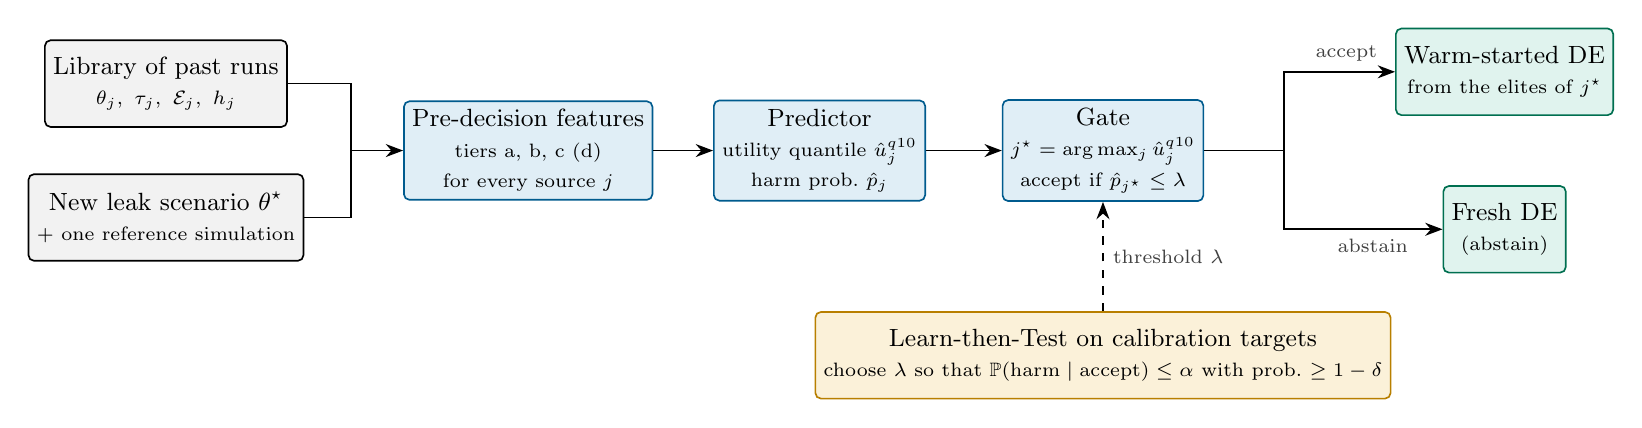
\begin{tikzpicture}[
  font=\small,
  box/.style={draw, rounded corners=2pt, align=center, minimum height=1.1cm, inner sep=3pt, line width=0.6pt},
  data/.style={box, fill=okgrey!10},
  ours/.style={box, fill=okblue!12, draw=okblue!80!black},
  opt/.style={box, fill=okgreen!12, draw=okgreen!70!black},
  arr/.style={-{Stealth[length=2.2mm]}, line width=0.6pt},
  lab/.style={font=\scriptsize, text=black!75}
]
\node[data] (lib) at (0, 0.85) {Library of past runs\\{\scriptsize $\theta_j,\ \tau_j,\ \mathcal{E}_j,\ h_j$}};
\node[data] (tgt) at (0,-0.85) {New leak scenario $\theta^\star$\\{\scriptsize + one reference simulation}};
\node[ours] (feat) at (4.6, 0) {Pre-decision features\\{\scriptsize tiers a, b, c (d)}\\{\scriptsize for every source $j$}};
\node[ours] (pred) at (8.3, 0) {Predictor\\{\scriptsize utility quantile $\hat u^{q10}_j$}\\{\scriptsize harm prob.\ $\hat p_j$}};
\node[ours] (gate) at (11.9, 0) {Gate\\{\scriptsize $j^\star=\arg\max_j \hat u^{q10}_j$}\\{\scriptsize accept if $\hat p_{j^\star}\le\lambda$}};
\node[opt] (warm) at (17.0, 1.0) {Warm-started DE\\{\scriptsize from the elites of $j^\star$}};
\node[opt] (fresh) at (17.0,-1.0) {Fresh DE\\{\scriptsize (abstain)}};
\node[box, fill=okorange!15, draw=okorange!80!black] (cal) at (11.9,-2.6)
  {Learn-then-Test on calibration targets\\{\scriptsize choose $\lambda$ so that $\Prob(\text{harm}\mid\text{accept})\le\alpha$ with prob.\ $\ge 1-\delta$}};
\coordinate (j) at (2.35, 0);
\draw[line width=0.6pt] (lib.east) -| (j);
\draw[line width=0.6pt] (tgt.east) -| (j);
\draw[arr] (j) -- (feat.west);
\draw[arr] (feat) -- (pred);
\draw[arr] (pred) -- (gate);
\coordinate (s) at (14.2, 0);
\draw[line width=0.6pt] (gate.east) -- (s);
\draw[arr] (s) |- node[lab, pos=0.78, above] {accept} (warm.west);
\draw[arr] (s) |- node[lab, pos=0.78, below] {abstain} (fresh.west);
\draw[arr, dashed] (cal.north -| gate.south) -- node[lab, right] {threshold $\lambda$} (gate.south);
\end{tikzpicture}}
\caption{The decision layer. For a new leak scenario, features are computed for every candidate source in the
library from information available before the search. A predictor ranks the sources by a lower quantile of their
utility and estimates each one's harm probability. The gate warm-starts DE from the top-ranked source only if its
harm probability is below a threshold $\lambda$ certified on held-out calibration targets; otherwise DE starts fresh.
The optimiser itself is not modified.}
\label{fig:pipeline}
\end{figure}

\subsection{Features available before the decision}\label{sec:features}

Every feature for a (target, source) pair is computed without running the target search. We group them in tiers so
that we can ask which kind of information matters.
\begin{description}[leftmargin=0pt]
  \item[Tier a, scenario facts (28 features).] Target and source scenario parameters and their differences; physical
        descriptors of the two leak nodes (elevation, local demand, hydraulic distance to the source of supply, pipe
        diameter, PRV zone); the leak share under a reference decision. The Euclidean distance between the
        standardised scenario vectors is one of these features.
  \item[Tier b, source trajectory (13).] Summaries of how the source run converged: improvement at 25/50/75\% of its
        budget, area under its best-so-far curve, decay of population diversity, feasible share, generation of the
        last improvement, spread of its elites.
  \item[Tier c, hydraulic signatures (78).] Statistics of pressure, leakage, energy and storage for the best
        solution of the source, for the target and source under a fixed mid-range reference decision, and of their difference, per
        time window. The target's signature costs one simulation. The cosine similarity between target and source
        reference pressure profiles is the kind of state similarity that SEETO-style methods use to select
        sources~\citep{fang2026seeto}.
  \item[Tier d, probe (optional).] Objective values of the $q$ injected elites evaluated on the target, compared with
        the random members of the initial population. This costs $q$ evaluations and is used only in the probe
        variant.
\end{description}

\subsection{Predictor}
We fit gradient-boosted trees (LightGBM~\citep{ke2017lightgbm}) with the quantile loss~\citep{koenker1978quantiles}
at levels 0.1, 0.5 and 0.9 for utility, and a gradient-boosted classifier with Platt scaling~\citep{platt1999probabilistic}
for the harm probability $\hat p^{\,\mathrm{harm}}$. Hyperparameters are chosen by cross-validation grouped by target, so
that no target appears in both the training and validation folds. Candidate sources are ranked by the 10\% quantile
$\hat u^{q10}_j$, a cautious estimate that penalises sources whose predicted benefit is uncertain.

\subsection{Risk-controlled gate}\label{sec:gate}

For each target the gate looks only at the top-ranked source $j^\star$ and accepts it if $\hat p_{j^\star}\le\lambda$.
The threshold $\lambda$ is chosen on calibration targets that were not used for training, one decision per target,
so that calibration points are independent. Following LTT~\citep{angelopoulos2025ltt}, each candidate threshold
$\lambda$ defines a null hypothesis
\[
  \mathcal{H}_\lambda:\ \Prob(\harm=1 \mid \hat p\le\lambda) > \alpha,
\]
which we test with the exact binomial tail: if $n_\lambda$ calibration targets are accepted and $k_\lambda$ of them
are harmful, the p-value is $\Prob(X\le k_\lambda)$ for $X\sim\mathrm{Bin}(n_\lambda,\alpha)$. Thresholds are tested in a
fixed order from strict to loose, and the procedure stops at the first non-rejection
(\cref{alg:ltt}). Because the order depends only on the predicted scores and never on the labels, fixed-sequence
testing controls the family-wise error rate at $\delta$, which gives:

\begin{proposition}[from \citep{angelopoulos2025ltt}]
If calibration and new targets are exchangeable, then with probability at least $1-\delta$ over the calibration
set, the harm rate among accepted transfers on new targets is at most $\alpha$.
\end{proposition}

One practical detail matters more than it looks. With very strict thresholds only one or two calibration targets are
accepted, and a binomial test on $n$ points with zero harms can only reject when $(1-\alpha)^n\le\delta$. Starting the
sequence at the strictest threshold therefore stops it immediately and the gate never transfers. We start the
sequence at the first threshold that accepts at least $n_{\min}=\lceil \ln\delta/\ln(1-\alpha)\rceil$ points
($n_{\min}=14$ for $\alpha=0.2$, $\delta=0.05$). This skips only hypotheses that could never be rejected; the order
still ignores the labels, so the guarantee is unchanged. We recorded this as a dated amendment to our pre-registration.

\begin{algorithm}[t]
\caption{Learn-then-Test threshold for the transfer gate}\label{alg:ltt}
\KwIn{calibration scores $\hat p_1,\dots,\hat p_n$ of the top-ranked sources; harm labels $\harm_1,\dots,\harm_n$; level $\alpha$; confidence $\delta$}
\KwOut{threshold $\lambda$, or \textsc{none} (always start fresh)}
$n_{\min}\leftarrow\lceil \ln\delta/\ln(1-\alpha)\rceil$;\quad $\lambda^\star\leftarrow\textsc{none}$\;
\ForEach{$\lambda$ in the sorted distinct values of $\hat p$ (strict $\to$ loose)}{
  $n_\lambda\leftarrow|\{i:\hat p_i\le\lambda\}|$;\quad $k_\lambda\leftarrow\sum_{i:\hat p_i\le\lambda}\harm_i$\;
  \lIf{$n_\lambda<n_{\min}$}{\textbf{continue}}
  \eIf{$F_{\mathrm{Bin}(n_\lambda,\alpha)}(k_\lambda)\le\delta$}{$\lambda^\star\leftarrow\lambda$}{\textbf{break}}
}
\Return{$\lambda^\star$}
\end{algorithm}

\subsection{Shift-aware gate}\label{sec:shiftgate}

The guarantee assumes that new targets look like the calibration targets. When the network changes, for example
because pipes are closed for repair, this may fail. Following the covariate-shift literature~\citep{tibshirani2019covariate,bickel2009discriminative},
we train a domain classifier to separate calibration targets from the new targets (whose features are known,
but whose labels are not) and weight each calibration point by its estimated density ratio
$w_i=\hat\Prob(\text{new}\mid z_i)/\hat\Prob(\text{cal}\mid z_i)$. The weighted harm rate is then tested at an effective
sample size $n_{\mathrm{eff}}=\min\bigl((\sum w_i)^2/\sum w_i^2,\ \sum w_i\bigr)$, Kish's
approximation~\citep{kish1965survey} capped by the total weight. We do not clip the weights: when the new targets
lie outside the calibration data, a few points receive large weights, $n_{\mathrm{eff}}$ collapses below $n_{\min}$,
and the gate abstains. This is an approximation rather than an exact finite-sample guarantee, and we treat it as
such; its purpose is to fail safe.

% ===========================================================================
\section{Experimental setup}\label{sec:setup}

\subsection{Networks, objective and optimiser}

\paragraph{Networks.} We use two benchmark networks, edited to support pressure management (\cref{tab:networks}).
\emph{Net3}, the EPANET example network, was given two PRV-fed zones by closing three pipes and inserting PRVs,
with its original controls removed. \emph{L-Town}, the 782-junction network of the BattLeDIM
competition~\citep{vrachimis2022battledim}, has one pump station and three PRVs. Both run with pressure-driven demand
(required pressure 20\,m) in EPANET~2.2 through WNTR~1.5~\citep{rossman2020epanet,klise2017wntr}. A leak is an
orifice emitter $q=C_dA\sqrt{2gp}$ at a junction. We call the toolkit directly through a compiled loop, which matches
WNTR's own EPANET simulator to within $10^{-5}$\,m in pressure and needs 3.6\,ms (Net3) or 28\,ms (L-Town) per 24-hour
simulation.

\paragraph{Objective.} $J_\theta(x)$ is a weighted sum of four terms over 24 hours: leak volume, energy cost under a
two-level time-of-use tariff, a pressure-shortfall penalty at demand nodes below 20\,m, and a penalty if total storage
at the end of the day is lower than at the start. The weights come from a normalisation rule fixed before any
transfer experiment (each term contributes comparably at the centre of the scenario space).

\paragraph{Optimiser and action.} We use our own DE/rand/1/bin~\citep{storn1997de} with an exact
evaluation budget; $F=0.4$, $CR=0.5$ and population size $N=20$ were tuned once on separate scenarios. The budget
$B$ was set by a pre-registered rule (median remaining regret against a $5B$ run between 3 and 20\%), giving $B=400$
on Net3 and $B=1000$ on L-Town. The transfer action injects the $k=3$ best distinct elites of the source, with 3\%
Gaussian noise, into $\rho=40\%$ of the initial population; $k$ and $\rho$ were fixed on a pilot before the main
campaign.

\begin{table}[t]
\centering\small
\caption{Networks and decision problems.}\label{tab:networks}
\begin{tabular}{@{}lcc@{}}
\toprule
 & Net3-PRV & L-Town-PRV \\
\midrule
Junctions & 94 & 782 \\
Controlled elements & 2 pumps, 2 PRVs & 1 pump station, 3 PRVs \\
Decision variables $D$ & 24 (4 per window $\times$ 6) & 24 (4 per window $\times$ 6) \\
PRV setting range (m) & 15--45 & 25--60 \\
Evaluation budget $B$ & 400 & 1000 \\
Simulation time per evaluation & 3.6\,ms & 28\,ms \\
\bottomrule
\end{tabular}
\end{table}

\subsection{Paired-run benchmark}

Scenarios are sampled from fixed ranges (leak area $2\cdot10^{-4}$ to $3\cdot10^{-3}$\,m$^2$ log-uniform, roughly 4 to
60\,L/s at 40\,m; demand multiplier 0.8--1.2; peak shift $\pm3$\,h; peak amplitude 0.8--1.2; initial tank level 30--80\%)
and split into four disjoint sets: \emph{library} scenarios, whose finished runs are the sources, and
\emph{training}, \emph{calibration} and \emph{test} targets. For each target we pick $S$ candidate sources from the
library, stratified by scenario distance (near, mid, far), and run fresh and warm DE $R$ times. Repeat $r$ of the fresh
run and of every warm run share the same seed, so the random part of the initial population and the DE random stream
are identical; only the injected elites differ. These common random numbers~\citep{law2015simulation} remove most of the
seed noise from the paired difference. \Cref{tab:experiments} lists the experiments.

\begin{table}[t]
\centering\small
\caption{Experiments. All targets are disjoint from the library. Pairs = targets $\times$ $S$ candidate sources.
$R$ = matched repeats per pair (test targets in brackets). $^{a}$Service pressure raised to 25\,m, or energy weight
doubled (40 targets each). $^{b}$One, two or three additional closed pipes (30 targets each).}\label{tab:experiments}
\setlength{\tabcolsep}{4.5pt}
\begin{tabular}{@{}llccccc@{}}
\toprule
 & Question & Network & Targets (train/cal/test) & $S$ & $R$ & Pairs \\
\midrule
E1 & main benchmark & Net3 & 60 / 80 / 40 & 6 & 8 (10) & 1\,080 \\
E2 & goal change$^{a}$ & Net3 & 80 & 6 & 8 & 480 \\
E3 & layout change$^{b}$ & Net3 & 90 & 6 & 8 & 540 \\
E4 & new network & L-Town & 90 / 70 / 20 & 3 & 4 & 540 \\
\midrule
 & optimiser check (GA instead of DE) & Net3 & 20 & 6 & 5 & 120 \\
\bottomrule
\end{tabular}
\end{table}

\Cref{fig:curves} shows what the labels look like. On the left the injected elites already sit near the optimum and
the warm run is ahead from the first evaluation; on the right they start in a poor, infeasible region and the warm
run never catches up within the budget.

\begin{figure}[t]
\centering
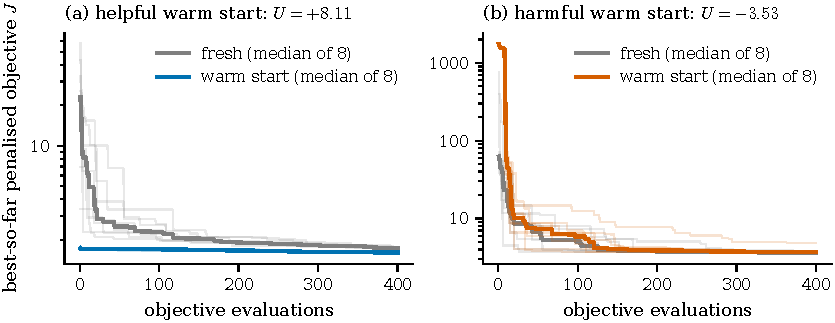
\includegraphics[width=\linewidth]{figures/fig_curves.pdf}
\caption{Best-so-far objective of fresh (grey) and warm-started (colour) DE on two Net3 targets; thin lines are the
individual matched repeats, thick lines their median. (a) The most helpful pair in E1. (b) The most harmful pair in
E1.}
\label{fig:curves}
\end{figure}

\subsection{Baselines and evaluation}

All methods choose among the same $S$ measured sources of a target (or start fresh), so their outcomes can be read
from the pair table without new runs, except where a method changes the search itself. Besides fresh DE and the
hindsight oracle (the best measured action per target), we compare: always transferring from the \emph{nearest}
scenario; \emph{similarity top-1}, which transfers from the source with the most similar hydraulic state; a
\emph{historical} rule based on mean training utilities in bins of scenario differences; and three adaptations of
recent sequential-transfer methods, re-implemented inside the same DE with their published hyperparameters:
\emph{SEETO-style} similarity-weighted multi-source injection~\citep{fang2026seeto}, \emph{BCKT-style} Bayesian
competition between sources during the run~\citep{lu2025bckt} (originally proposed for surrogate-assisted multi-task
search, here applied with finished sources), and a \emph{PMTO-style} task model that maps
scenario parameters to an injected solution~\citep{wei2025pmto}. These are not the authors' code; we document every
change in the repository. Comparisons are made over test targets with Wilcoxon signed-rank tests~\citep{wilcoxon1945individual}
and Holm's correction~\citep{holm1979simple}, after a Friedman test~\citep{friedman1937ranks}; confidence intervals are
percentile bootstraps over targets, and rates of harm carry Clopper--Pearson intervals~\citep{clopper1934binomial}.

\paragraph{Pre-registration.} Hypotheses, splits, the label definition, $\varepsilon$, $\alpha\in\{0.1,0.2\}$, $\delta=0.05$
and the analysis plan were written down and frozen before the main campaign, in the spirit of
\citet{nosek2018preregistration}. Every later change is recorded as a dated amendment, and the test targets were read
once, at the end. Following benchmarking advice in evolutionary computation~\citep{bartzbeielstein2020benchmarking},
we report results that went against our hypotheses alongside those that supported them.

% ===========================================================================
\section{Results}\label{sec:results}

\subsection{What the benchmark shows}\label{sec:res-bench}

On Net3 with DE, warm starts are usually good: 80.4\% of the 1\,080 pairs are helpful ($U>\varepsilon$), 16.8\% neutral
and only 2.9\% harmful, with a mean utility of 1.48 (\cref{fig:utility}). L-Town is a different place. Only 60.2\% of
pairs help, 16.1\% harm, and the distribution of $U$ has a long left tail. On both networks harm grows with the
scenario distance between source and target, but distance alone is a weak signal: even among the nearest third of
sources, 8.3\% of L-Town pairs are harmful. Label noise is modest; the median standard error of a pair's utility is
about a third of the spread of utilities across pairs (0.32 on Net3, 0.23 on L-Town).

\begin{figure}[t]
\centering
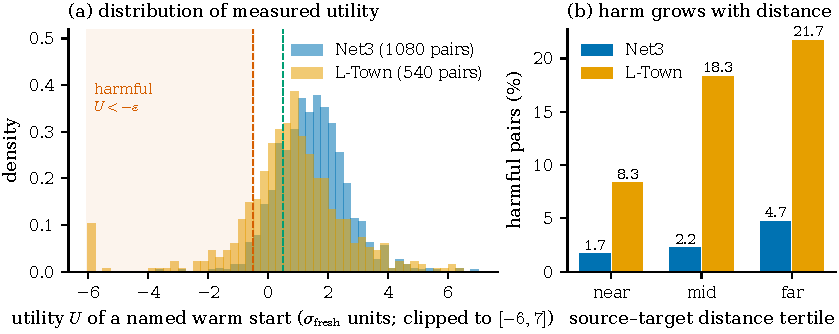
\includegraphics[width=\linewidth]{figures/fig_utility.pdf}
\caption{(a) Measured utility of all named warm starts on Net3 (E1) and L-Town (E4), in units of the fresh-run
standard deviation; dashed lines at $\pm\varepsilon$. (b) Share of harmful pairs by scenario-distance tertile.}
\label{fig:utility}
\end{figure}

\subsection{Utility is predictable; similarity is not}\label{sec:res-predict}

\Cref{fig:predict}a reports the out-of-fold rank correlation between predicted and measured utility on the 360 E1
training pairs, for predictors that see different tiers of features. The hydraulic-state similarity that a
SEETO-style method uses has a Spearman correlation of 0.05 [$-0.07$, 0.17] with the measured utility, and scenario
distance $-0.07$. Scenario facts alone reach 0.51, all zero-shot tiers 0.58 [0.41, 0.69], and adding the probe of the
injected elites 0.67 [0.56, 0.75]. The difference between the full zero-shot model and similarity is 0.53 [0.36, 0.68].

Which information carries this? Permuting one tier at a time inside the zero-shot model costs 0.39 in Spearman for
scenario facts, 0.18 for hydraulic signatures and 0.005 for the source trajectory, and shuffling the order of
generations in the trajectory features changes nothing (difference $-0.002$ [$-0.016$, 0.013]). The value lies in
the physics of the two leak events, not in how the source search happened to unfold. As a check on leakage, the same
pipeline with labels permuted across targets drops to 0.10.

Harm itself is harder. With only five harmful pairs among the Net3 training data, no model separates them
reliably (\cref{fig:predict}b, crosses). On L-Town, where harm is common, the harm classifier is useful: with 90
training targets its out-of-fold AUROC is 0.84 [0.68, 0.95], and 0.79 on the held-out test targets.

\begin{figure}[t]
\centering
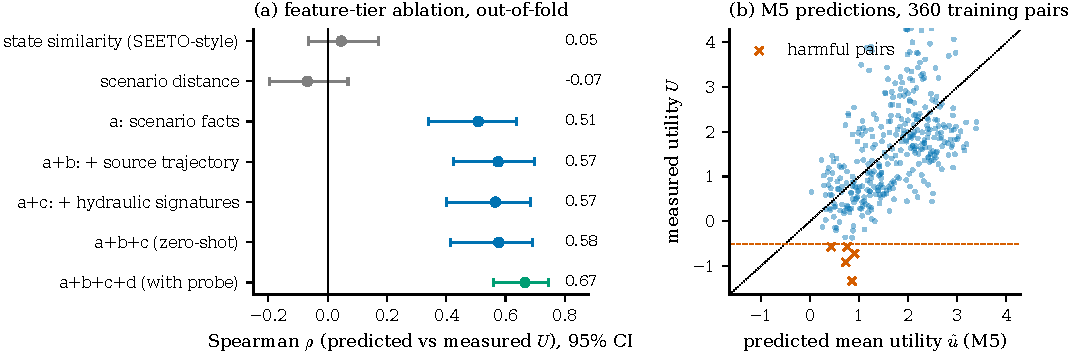
\includegraphics[width=\linewidth]{figures/fig_predict.pdf}
\caption{(a) Out-of-fold Spearman correlation between predicted and measured utility on Net3 training targets, with
95\% bootstrap intervals over targets. Grey: single similarity or distance features. (b) Predicted against measured
utility for the zero-shot model; crosses mark harmful pairs.}
\label{fig:predict}
\end{figure}

\subsection{Decisions on the same network}\label{sec:res-gate}

\paragraph{The bound holds.} Over 200 random re-splits of the E1 calibration and test targets, the realised harm rate
among accepted transfers stays at or below $\alpha$ in 100\% of splits for every $\alpha\ge0.10$, and in 95.5\% at
$\alpha=0.05$, consistent with $\delta=0.05$ (\cref{fig:gate}a). The price shows up only at the strictest level: at
$\alpha=0.05$ the gate abstains on 65\% of targets on average, because certifying that level needs at least
$n_{\min}=59$ accepted calibration targets with almost no harm among them, which a calibration set of 80 targets
often cannot supply (\cref{fig:gate}b).

\paragraph{The test set.} On the 40 untouched test targets, read once, the gate at $\alpha=0.2$ transfers on 39
and abstains on one. None of the 39 transfers is harmful (Clopper--Pearson upper bound 9.0\%). Its mean utility
is 1.74, or 87.5\% of what the hindsight oracle achieves (\cref{tab:policies}). In physical terms, the gated warm start
ends the day with 0.8\% less leaked volume and 13\% lower energy cost than fresh DE at the same budget, and it saves
on average 233 of the 400 evaluations needed to reach the fresh run's final quality.

\begin{figure}[t]
\centering
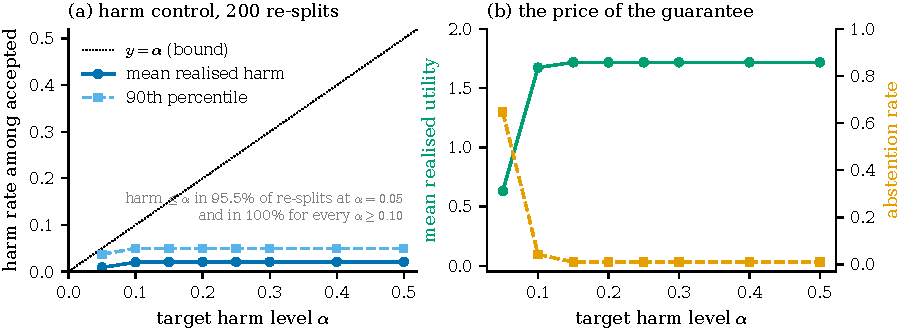
\includegraphics[width=\linewidth]{figures/fig_gate.pdf}
\caption{The Learn-then-Test gate on Net3, over 200 random calibration/test re-splits. (a) Realised harm rate among
accepted transfers against the nominal level. (b) Mean utility and abstention rate.}
\label{fig:gate}
\end{figure}

\begin{table}[t]
\centering\small
\caption{Policies on the 40 Net3 test targets (E1). Utility in fresh-run standard deviations, 95\% bootstrap CI over
targets. $p$: Holm-corrected Wilcoxon test against the gate. Harm: share of harmful transfers among those made.
Friedman test over all policies: $\chi^2=222.5$, $p<10^{-40}$.}\label{tab:policies}
\setlength{\tabcolsep}{5pt}
\begin{tabular}{@{}lcccc@{}}
\toprule
Policy & Mean $U$ [95\% CI] & $p$ vs gate & Harm & \% of oracle \\
\midrule
Oracle (hindsight)                      & 1.99 [1.72, 2.26] & --     & 0.0\% & 100.0 \\
\midrule
\textbf{Gate, $\alpha=0.2$ (ours)}      & \textbf{1.74} [1.44, 2.03] & -- & 0.0\% & 87.5 \\
Learned ranking without gate (ours)     & 1.77 [1.49, 2.05] & 1.00 & 0.0\% & 89.1 \\
Gate with probe, $q=8$ (ours)           & 1.74 [1.44, 2.04] & 1.00 & 0.0\% & 87.5 \\
\midrule
SEETO-style multi-source~\citep{fang2026seeto} & 1.75 [1.42, 2.05] & 1.00 & 7.5\% & 87.7 \\
Similarity top-1                         & 1.68 [1.38, 1.98] & 0.66 & 2.5\% & 84.4 \\
Historical rule                          & 1.61 [1.30, 1.89] & 0.45 & 2.5\% & 80.6 \\
Nearest scenario                         & 1.54 [1.24, 1.83] & 0.039 & 0.0\% & 77.3 \\
PMTO-style task model~\citep{wei2025pmto} & 1.49 [1.26, 1.73] & 0.039 & 0.0\% & 75.0 \\
BCKT-style competition~\citep{lu2025bckt} & 1.02 [0.78, 1.24] & $<0.001$ & 5.0\% & 51.2 \\
Fresh DE                                 & 0.00              & $<0.001$ & --    & 0.0 \\
\bottomrule
\end{tabular}
\end{table}

\paragraph{Against the baselines.} The gate is significantly better than always taking the nearest scenario, the
PMTO-style task model and BCKT-style competition. It is statistically indistinguishable from SEETO-style
multi-source injection and from similarity top-1. We want to be plain about this: on Net3, where nearly every warm
start helps, picking a reasonable source is most of the battle and the gate's abstain option almost never matters.
The difference is in what the operator is told. The SEETO-style policy made three harmful transfers out of 40 and
gives no statement about how often it will; the gate made none and comes with a bound. The probe, which spends eight
evaluations to look at the injected elites before deciding, improves prediction (\cref{sec:res-predict}) but changed
no decision on the test set.

\subsection{When the world shifts}\label{sec:res-shift}

The guarantee rests on new targets being exchangeable with the calibration targets. We tested three ways in which
that can fail, keeping the predictor and gate trained on E1 frozen.

\paragraph{Goal change (E2).} Raising the service pressure to 25\,m, or doubling the weight of energy, changes the
objective but not the network. The frozen predictor keeps its accuracy (Spearman 0.61 and 0.63) and the frozen gate
stays within $\alpha$ (one harmful transfer in 19, and none in 20).

\paragraph{Layout change (E3).} Closing pipes changes the hydraulics that the features describe. With one, two and three
closed pipes the share of harmful pairs rises from 8.3\% to 13.3\% and 17.8\%, the predictor's Spearman falls from 0.57
to 0.28 and 0.12, and the frozen gate keeps transferring on every target. With three closures its realised harm
rate is 23.3\% against a nominal 20\% (\cref{fig:shift}). The guarantee has not been violated in a technical sense,
because its assumption no longer holds, but an operator would not care about that distinction.

\paragraph{Shift-aware gate.} The density-ratio-weighted gate of \cref{sec:shiftgate} sees the shift coming: the domain
classifier separates calibration from E3 targets with AUC 0.54, 0.80 and 0.89 for one, two and three closures. At
$\alpha=0.2$ it behaves like the frozen gate for one and two closures and abstains on all 30 targets with three,
bringing the harm among accepted transfers to zero (\cref{tab:shift}). On the unshifted E1 test set its decisions are
identical to the plain gate's (39 of 40 transfers, $U=1.74$), and it refuses to carry the Net3 gate over to L-Town
(domain AUC 0.95). The cost is visible too: the 25\,m pressure goal of E2 is perfectly detectable (AUC 1.00) but
harmless, and there the shift-aware gate abstains and gives up a utility of 1.38 that the frozen gate would have
collected safely. Detecting a shift is not the same as detecting harm.

\begin{figure}[t]
\centering
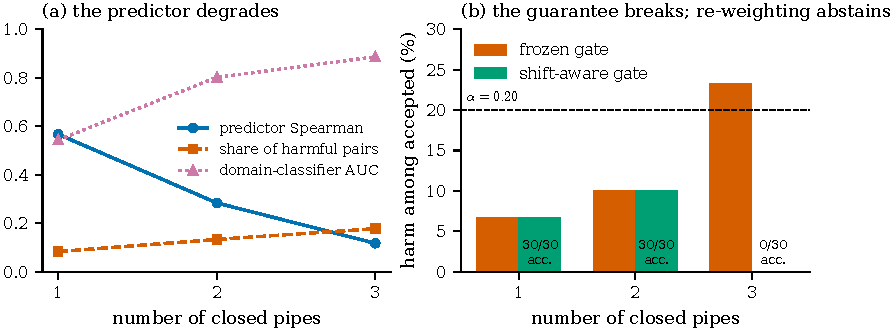
\includegraphics[width=\linewidth]{figures/fig_shift.pdf}
\caption{Layout shift (E3), with the predictor and gate frozen from E1. (a) Predictor accuracy falls and harm rises
as more pipes are closed; the domain classifier notices. (b) Harm among accepted transfers at $\alpha=0.2$; labels
give the number of targets the shift-aware gate accepted.}
\label{fig:shift}
\end{figure}

\begin{table}[t]
\centering\small
\caption{Frozen and shift-aware gates under shift ($\alpha=0.2$). Acc.: accepted targets. Harm: among accepted.
$U$: mean realised utility over all targets (abstain counts as 0).}\label{tab:shift}
\setlength{\tabcolsep}{4.5pt}
\begin{tabular}{@{}llccccccc@{}}
\toprule
 & & & \multicolumn{3}{c}{Frozen gate} & \multicolumn{3}{c}{Shift-aware gate} \\
\cmidrule(lr){4-6}\cmidrule(l){7-9}
Exp. & Condition & Domain AUC & Acc. & Harm & $U$ & Acc. & Harm & $U$ \\
\midrule
E1 & no shift (test)        & 0.43 & 39/40 & 0.0\%  & 1.74 & 39/40 & 0.0\% & 1.74 \\
E2 & service pressure 25\,m & 1.00 & 19/20 & 5.3\%  & 1.38 & 0/20  & --    & 0.00 \\
E2 & energy weight $\times2$ & 0.43 & 20/20 & 0.0\%  & 1.46 & 20/20 & 0.0\% & 1.46 \\
E3 & 1 closed pipe          & 0.54 & 30/30 & 6.7\%  & 1.15 & 30/30 & 6.7\% & 1.15 \\
E3 & 2 closed pipes         & 0.80 & 30/30 & 10.0\% & 0.42 & 30/30 & 10.0\% & 0.42 \\
E3 & 3 closed pipes         & 0.89 & 30/30 & \textbf{23.3\%} & 0.01 & 0/30 & -- & 0.00 \\
E4 & new network (L-Town)   & 0.95 & 20/20 & 5.0\%  & 1.47 & 0/20  & --    & 0.00 \\
\bottomrule
\end{tabular}
\end{table}

\subsection{A network where harm is common}\label{sec:res-ltown}

L-Town is where a decision layer should earn its keep, since one warm start in six is harmful. The Net3 predictor
does not transfer to it (Spearman 0.08), so we trained on L-Town itself and studied how results change with the
amount of local data. With 30 training targets, a learned ranking without a gate reaches $U=1.61$ (72\% of the
oracle); with 90 it reaches 1.79 (80.5\%), with one harmful decision in 20 test targets. Similarity top-1 reaches 1.30
and the nearest scenario 0.79 at 30 targets.

Certification is another matter (\cref{fig:ltown}). With 70 calibration targets and $\alpha=0.2$, the gate holds its
bound in 99\% of 200 re-splits, but abstains on 61\% of targets on average and keeps a mean utility of 0.43, about a
quarter of the ungated ranking. It becomes useful only from $\alpha=0.25$. Borrowing Net3 data does not help: a model
trained on both networks separates harm well in cross-validation (AUROC 0.89), but its scores are less sharp on the
L-Town calibration set and the gate abstains even more. Calibrating on Net3 and L-Town targets together does
``certify'' L-Town, but only by borrowing Net3's low harm rate, and the shift-aware test rejects exactly that.

The lesson is about sample size, not modelling. With a true harm rate among top-ranked sources of a few percent and
$\alpha=0.2$, a binomial certificate at $\delta=0.05$ needs tens of accepted, mostly harm-free calibration targets in the
region where the gate accepts. A utility has to collect that evidence before it can promise anything.

\begin{figure}[t]
\centering
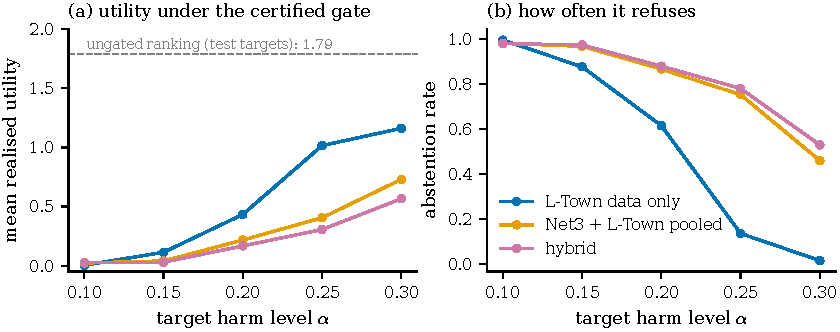
\includegraphics[width=\linewidth]{figures/fig_ltown.pdf}
\caption{The certified gate on L-Town (90 training, 70 calibration targets), mean over 200 re-splits. (a) Realised
utility; the dashed line is the ungated ranking on the test targets. (b) Abstention rate. Colours: training data of
the predictor.}
\label{fig:ltown}
\end{figure}

\subsection{What did not work, and what limits everything}\label{sec:res-robust}

\paragraph{Changing the optimiser.} We repeated 120 Net3 pairs with a real-coded genetic algorithm (SBX crossover~\citep{deb1995sbx},
polynomial mutation, $(\mu+\lambda)$ selection) instead of DE, with the same budget, action and seeds. The share of
harmful pairs rises from 1.7\% to 13.3\%, the mean utility falls from 1.51 to 0.44, and the utilities of the same pairs
under the two optimisers are essentially unrelated (Spearman 0.08, \cref{fig:ga}). Whether a past run helps is a
property of the source, the target \emph{and} the optimiser. Every predictor in this paper is specific to DE, and we
expect the same to hold for other methods.

\begin{figure}[t]
\centering
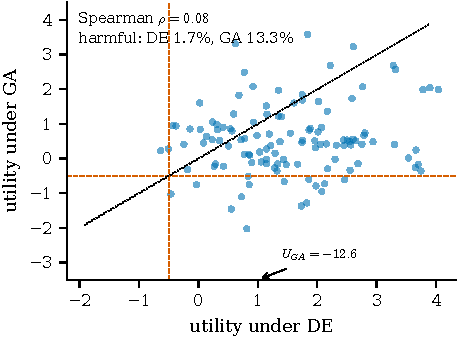
\includegraphics[width=0.5\linewidth]{figures/fig_ga.pdf}
\caption{Utility of the same 120 source--target pairs under DE and a genetic algorithm. Dashed lines: harm threshold
$-\varepsilon$.}
\label{fig:ga}
\end{figure}

\paragraph{Trajectory monitoring.} A natural idea is to start the warm run, watch it for a few generations, and abort
to a fresh run if it looks bad. Under common random numbers the outcome of such a policy can be computed exactly
from the logged runs, so we tested it without new simulations, comparing the warm run's progress at generation
$g\in\{1,2,4,8\}$ with the progress expected from a fresh run. It did not help. A monitor tuned for utility without
any guarantee converged to never aborting ($U=1.61$ against 1.61 on L-Town, 1.77 against 1.77 on Net3), and a
risk-controlled monitor could not certify anything on L-Town and aborted every run, paying the restart cost each
time. Early progress does not separate harmful warm starts from helpful ones well enough to repay the evaluations it
costs to find out.

\paragraph{Sensitivity.} The picture depends on the design choices in the expected direction. Injecting fewer
elites ($\rho=0.1$) lowers the mean utility to 0.99 and raises harm to 5.8\%; a smaller budget ($B=200$) makes warm
starts worth more ($U=2.38$) and a larger one ($B=600$) worth less (1.23). The gate is fragile when the harm model is
weak: with $\varepsilon=1.0$ only one training pair is harmful, the single harmful calibration target lands inside the
first testable threshold, and the fixed sequence stops at once, so the gate never transfers.

\paragraph{Cost.} Labelling the 360 training pairs took 1.34 million evaluations. At 233 evaluations saved per task,
the library pays for itself after roughly 5\,800 future tasks. With simulations that take milliseconds this is not
worth it, and we do not claim otherwise. The argument for the approach rests on settings where an evaluation is
expensive and the paired labels can be collected as a by-product of normal operation.

% ===========================================================================
\section{Discussion}\label{sec:discussion}

\paragraph{What we think holds.} Three messages survive all the checks we could run. First, the benefit of reusing a
named past run can be predicted from physical information available before the run, while the similarity on which
most source-selection rules rest says almost nothing about it. Second, a finite-sample harm bound is easy to keep
where harm is rare and expensive to keep where harm is common: on L-Town the ranking alone captures 80\% of the
oracle with 5\% harmful decisions, while the certified gate gives up most of that to make its promise with 70
calibration cases. For practice this suggests a learned ranking paired with a gate whose strictness matches the
size of the calibration set, tightened as evidence accumulates. Third, exchangeability is the weak point. A frozen
gate is not safe after the network changes, and a shift-aware gate is safe only because it refuses to act.

\paragraph{Limitations.} The study has clear limits. It uses two benchmark networks and one transfer action;
simulations are cheap, so savings are measured in evaluations, not in hours. The labels come from 4 to 10 repeats per
pair, so the guarantee is relative to an estimated harm label. Our baselines are re-implementations, not the
authors' code; we fixed their hyperparameters at published values and spent no tuning budget on them, which may
understate them. The shift-aware test uses an effective sample size and is an approximation. Finally, the GA result
means that every quantitative statement here is conditional on DE.

\paragraph{What we would do next.} The obvious step is an expensive simulator, or a real utility's model, where a
saved evaluation matters and where calibration cases accumulate during operation. Online versions of the gate that
update $\lambda$ as labelled cases arrive, and harm predictors that look at the injected elites more directly, seem
the most promising ways to reduce the cost of certification on networks like L-Town.

% ===========================================================================
\section{Conclusion}\label{sec:conclusion}

Reusing a past optimisation run is not automatically a good idea, and whether it is can be estimated before
committing the budget. We framed warm-starting in sequential evolutionary transfer as a decision with an operator-chosen
cap on harm, built a paired benchmark to measure it on two water networks, and showed that a learned predictor
with a Learn-then-Test gate gives useful, certified decisions where harm is rare, honest but costly ones where harm is
common, and a safe refusal under layout shift when the calibration is reweighted. We hope the benchmark, and the
negative results reported alongside the positive ones, make it easier for others to ask the same question about
their own optimisers.

% ===========================================================================
\section*{Code and data availability}
All code, edited network files, scenario manifests, paired-run tables, pre-registration and decision log are
available at \url{https://github.com/likhith1253/watercdn}. Every number in this paper is generated from files in
that repository; \texttt{scripts/reproduce.py} reruns the full study and \texttt{scripts/paper\_figures.py} redraws
the figures.

% \section*{Acknowledgements}
% Funding, people, compute. Also state here how AI tools were used, if at all, as many venues now ask.

\bibliographystyle{plainnat}
\bibliography{references}

% ===========================================================================
\appendix
\section{Implementation details}\label{app:details}

\begin{table}[h]
\centering\small
\caption{Frozen settings (from the pre-registration and its amendments).}\label{tab:settings}
\begin{tabular}{@{}l>{\raggedright\arraybackslash}p{0.7\linewidth}@{}}
\toprule
Setting & Value \\
\midrule
DE & rand/1/bin, $F=0.4$, $CR=0.5$, $N=20$, exact budget $B$ \\
Budget rule & median regret vs.\ a $5B$ run in [3\%, 20\%] (Net3: 9.5\%, $B=400$; L-Town: 6.3\%, $B=1000$) \\
Transfer action & top-$k=3$ distinct elites, noise 3\% of range, $\rho=0.4$ of initial population \\
Harm tolerance & $\varepsilon=0.5$ fresh-run standard deviations \\
Gate & $\alpha\in\{0.10, 0.20\}$, $\delta=0.05$, fixed-sequence LTT starting at $n_{\min}$ \\
Predictor & LightGBM; quantiles 0.1/0.5/0.9; harm classifier with Platt scaling \\
Cross-validation & 5 folds grouped by target, on training targets only \\
Re-splits & 200 random calibration/test splits of the pooled calibration and test targets \\
Simulator & EPANET 2.2 (WNTR 1.5.0), pressure-driven demand, 1\,h steps, 24\,h \\
\bottomrule
\end{tabular}
\end{table}

\paragraph{Unattainable targets.} For 12\% of Net3 targets no feasible operation exists within the scenario ranges
(even a run of $5B$ evaluations does not find one); their utilities are driven by penalty terms. We kept them,
because an operator would face them too.

\paragraph{Reproducibility check.} Re-running 700 randomly chosen runs after later code changes reproduced every
best-so-far curve bit for bit.

\end{document}
